\chapter{Математическая модель и численный метод для повышения разрешения изображений мигающей флуоресцентной микроскопии}\label{ch:ch1}

Флуоресцентная микроскопия обладает рядом достоинств, среди которых высокая контрастность изображений и возможность маркировки разных структур разными красителями. Благодаря этому данный вид микроскопии получил широкое распространение. Однако разрешающая способность микроскопа ограничена дифракцией, а использование оптического диапазона длин волн делает разрешающую способность изображений флуоресцентной микроскопии недостаточной для ряда современных задач. В связи с этим развиваются различные подходы решения данной проблемы.

Двумя основными направлениями методов повышения разрешающей способности микроскопов являются восстановление размытых изображений и повышение разрешения изображений. Получение изображения с более высоким разрешением необходимо, если сам микроскоп не обеспечивает должного увеличения для различения мелких объектов. Если же микроскоп имеет сильное увеличение, то основным препятствием становится дифракция света, поэтому в таком случае задача устранения размытия выходит на передний план.

Использование стохастически мигающих флуорофоров даёт дополнительную информацию для анализа изображения и позволяет выделять сигналы отдельных участков объекта или отдельных флуорофоров на фоне друг друга при наличии временной серии изображений. Такой подход не требует специального оборудования, поэтому в настоящее время получил широкое распространение и продолжает активно развиваться~\cite{мишин2019флуоресцентная}. В этой главе рассматриваются именно такие методы повышения качества изображений флуоресцентной микроскопии на основе анализа временной серии снимков образца, подсвеченного стохастически мигающим красителем. Пример последовательных кадров из рассматриваемых серий изображений представлен на Рис.~\ref{fig:blinking-samples}.

\begin{figure}[ht]
	\centerfloat{
		\hfill
		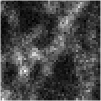
\includegraphics[width=0.18\textwidth]{blinking-1-6a.png}
		\hfill
		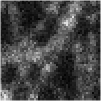
\includegraphics[width=0.18\textwidth]{blinking-1-6b.png}
		\hfill
		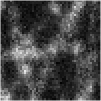
\includegraphics[width=0.18\textwidth]{blinking-1-6c.png}
		\hfill
		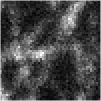
\includegraphics[width=0.18\textwidth]{blinking-1-6d.png}
		\hfill
		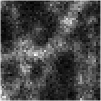
\includegraphics[width=0.18\textwidth]{blinking-1-6e.png}
		\hfill
	}
	\caption{Пример серии изображений, полученных с использованием мигающих флуорофоров}
	\label{fig:blinking-samples}
\end{figure}

В последние годы для этой области микроскопии было разработано множество алгоритмов, основанных на различных подходах, для решения задачи построения резкого изображения с высоким разрешением на основе серии снимков. В частности, алгоритмы PALM~\cite{betzig2006imaging} и STORM~\cite{rust2006sub} использует редко мигающие красители, чтобы находить центры отдельных пятен в каждом кадре и строить карту молекул флуорофора. Ограничением является требование низкой частоты мигания молекул и длинных серий снимков для визуализации всех участков изучаемого объекта.

Метод SOFI~\cite{dertinger2009fast, dertinger2010achieving} использует корреляцию и полуинварианты (см.~\cite{75086, малахов1978кумулянтный}) пикселей для уменьшения размытия и увеличения разрешения изображения. Однако он чувствителен к шуму, поэтому требует длинных последовательностей данных, а также этапа устранения размытия.

В то время как полуинварианты, используемые в SOFI, оценивают только часть ковариационной матрицы серии изображений, SPARCOM~\cite{Solomon:18} полностью использует эту матрицу и использует предположение о разреженности в пространстве корреляций сигналов флуорофоров для достижения более высокого пространственного разрешения и уменьшения требований к длине последовательности изображений.

Метод MUSICAL~\cite{agarwal2016multiple} вдохновлён алгоритмом обработки радиолокационных сигналов MUSIC~\cite{schmidt1986multiple}. Он использует собственные вектора серии изображений для построения карты флуорофоров с высоким разрешением.

Другой подход предложен авторами 3B~\cite{cox2012bayesian}. Их метод байесовского анализа мигания и выгорания моделирует изменение состояний флуорофоров и вычисляет расположение молекул. Однако его вычислительная сложность очень высока, и для практического использования этого алгоритма требуется кластерный компьютер.

Для этой задачи также разработаны методы, основанные на глубоком обучении. Например, свёрточная нейтральная сеть Deep"~STORM~\cite{Nehme:18} основана на архитектуре кодировщик"=декодировщик и напрямую создаёт изображения с высоким разрешением, тогда как метод DLBI~\cite{10.1093/bioinformatics/bty241} сочетает в себе как глубокое обучение, так и байесовский вывод, который уточняет результат нейронной сети.

Однако проблема всё ещё остаётся открытой, и требуется более высокая производительность алгоритмов улучшения изображения. Поэтому в данной диссертационной работе разработан численный метод реконструкции изображения повышенного разрешения и проведено сравнение его эффективности с некоторыми другими современными методами.

\section{Математическая модель искажения изображения}

Модель искажения изображения флуоресцентной микроскопии имеет вид:

\begin{equation*}
	y_{ij} = \left(Kx+n\right)_{ij},\quad K=DB,
\end{equation*}

\noindent где $x$ "--- исходное резкое изображение высокого разрешения, $y$ "--- наблюдаемое изображение, $K$ "--- оператор размытия и понижения разрешения, действие которого эквивалентно последовательному действию оператора размытия $B$ и оператора понижения разрешения $D$ (производящего, например, усреднение групп соседних пикселей или простое прореживание пиксельной сетки изображения), а $n$ "--- аддитивный шум с нормальным распределением.

\subsection{Модель размытия изображения} \label{sec:image-blur-model}

Рассматриваемая модель размытия изображения имеет вид свёртки изображения с ядром размытия:

\begin{equation*}
%	I^\prime \left( x, y \right)=\left(K\ast I+N\right)\left(x,y\right)=\int_{-\infty}^{\infty}\int_{-\infty}^{\infty}{K\left(s,t\right)\ I\left(x-s,y-t\right)\ ds\ dt}+N(x,y),
	x^\prime \left(p, q\right) = \left(B \ast x\right) \left(p, q\right) = \int_{-\infty}^{\infty}\int_{-\infty}^{\infty}{B\left(s,t\right)\ x\left(p-s,q-t\right)\ ds\ dt},
\end{equation*}

\noindent где $x$ "--- исходное резкое изображение, $x^\prime$ "--- искажённое изображение, $B$ "--- ядро размытия (англ.~point spread function, PSF), что в дискретном случае принимает вид:

\begin{equation*}
	x^\prime_{i,j} = \left(B \ast x\right)_{i,j} = \sum_{k=-\infty}^{\infty} \sum_{p=-\infty}^{\infty}{B_{k,p}\ x_{i-k,j-p}}.
\end{equation*}

\subsection{Модель ядра размытия} \label{sec:microscope-psf}

Получившее широкое распространение конфокальные лазерные микроскопы позволяют, сканируя образец лазерным лучом, возбуждать молекулы флуорофора в малых областях образца и получать в итоге более чёткое изображение, чем  при подсветке всего образца сразу. Кроме того, флуоресцентное излучение со смежных слоёв образца, находящихся не в фокусе объектива, частично отсекается точечной диафрагмой, расположенной перед приёмником света. Базовая схема такого микроскопа представлена на Рис.~\ref{fig:scanning-microscope-scheme}.

\begin{figure}[ht]
	\centerfloat{
		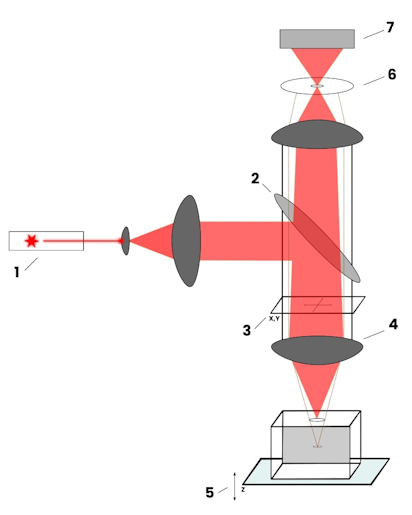
\includegraphics[height=0.4\textheight]{scanning-microscope-scheme.png}
	}
	\caption{Базовая схема конфокального лазерного сканирующего микроскопа. 1 "--- источник лазерного излучения; 2 "--- дихроичное зеркало, отражающее излучение с определённой длиной волны; 3 "--- механизм управления направлением луча лазера; 4 "--- линза объектива; 5 "--- механизм управления расстоянием от объектива до образца; 6 "--- точечная диафрагма; 7 "--- детектор флуоресцентного излучения.}
	\label{fig:scanning-microscope-scheme}
\end{figure}

%Благодаря поточечной подсветке, ядро размытия в лазерном сканирующем микроскопе $PSF_{eff}\left(r\right)$ определяется произведением ядра размытия лазерного луча подсветки образца $PSF_{exc}\left(r,r_{0,exc}\right)$ и ядра размытия объектива $PSF_{em}\left(r,r_{0,em}\right)$. Каждое из этих ядер симметрично и задаётся формулами:

Благодаря поточечной подсветке, ядро размытия в лазерном сканирующем микроскопе $PSF_{eff}$ определяется произведением ядра размытия лазерного луча подсветки образца $PSF_{exc}$ и ядра размытия объектива $PSF_{em}$ (см.~\cite{weisshart2014basic}). Каждое из этих ядер симметрично и задаётся формулами:

\begin{align*}
	&PSF\left(r, r_0\right) = I_0 \cdot \left(\frac{2\cdot J_1\left(v\right)}{v}\right)^2, \\
	&v=\frac{2\cdot\pi\cdot A\cdot\left|r-r_0\right|}{\lambda}, \\
	&J_1(v)=\sum_{n=0}^{\infty}{\left(-1\right)^n\frac{x^{2n+1}}{2^{2n+1}n!\left(n+1\right)!}},
\end{align*}

\noindent где $I_0$ "--- нормирующий множитель, $J_1$ "--- функция Бесселя первого рода первого порядка, $A$ "--- числовая апертура фокусирующей линзы, $r$ "--- точка в плоскости изображения, $r_0$ "--- центр ядра размытия в плоскости изображения, $\lambda$ "--- длина волны лазера подсветки или флуоресцентного излучения.

Характер отдельного ядра размытия $PSF\left(r, r_0\right)$ определён дифракцией света, наиболее освещённая центральная область плоскости изображения ядра называется диском Эйри. Расстояние $d_a$ между ближайшими к центру этого ядра нулями называется диаметром диска Эйри (англ.~airy unit, AU) и равно $\frac{\mu\cdot \lambda}{\pi \cdot A}$, где $\mu$ "--- наименьший положительный нуль функции Бесселя первого рода первого порядка.

Итоговое ядро размытия получаемого микроскопом изображения имеет вид $PSF_{eff}\left(r\right)=PSF_{exc}\left(r,r_{0,exc}\right)\cdot PSF_{em}\left(r,r_{0,em}\right)$, где $r$ "--- точка на изображении, $r_{0,exc}$, $r_{0,em}$ "--- центры ядер размытия лазера подсветки и флуоресцентного излучения соответственно (см.~Рис.~\ref{fig:blinking-psf}).

\section{Описание данных}

\subsection{Источники данных}

Искусственные данные были подготовлены с помощью инструмента для симуляции процесса получения серий снимков мигающей флуоресцентной микроскопии SOFI Simulation Tool~\cite{10.1371/journal.pone.0161602}, модифицированном для получения структуры в виде сходящихся отрезков.

Экспериментальные данные были получены в сотрудничестве с биологами Токийского университета с помощью микроскопа Zeiss~LSM~880 с детектором Airyscan~\cite{weisshart2014basic}, состоящем из 32 сенсоров, и мигающего флуоресцентного красителя HMSiR~\cite{uno2014spontaneously}. Серия снимков представляла собой 32 синхронных серии с разных сенсоров микроскопа, которые были предварительно совмещены.

\subsection{Детектор Airyscan}

%В данной главе задача повышения качества снимков решается для лазерного сканирующего микроскопа Zeiss~LSM~880, на котором установлен объектив с шестидесятикратным увеличением и детектор Airyscan~\cite{weisshart2014basic}, состоящий из 32 сенсоров, изображения с которых совмещаются для предварительного повышения резкости итогового снимка. Для такой системы задача устранения размытия становится крайне важной.

Так как итоговое ядро размытия лазерного сканирующего микроскопа представляет собой произведение ядра размытия луча подсветки и ядра размытия излучения объекта (см.~п.~\ref{sec:microscope-psf}), то при смещении детектора излучённого света в сторону от оптической оси микроскопа результирующее ядро размытия будет меняться, становясь более узким в центральной части, но приобретая более весомый <<хвост>>, как показано на Рис.~\ref{fig:blinking-psf-displacement}. На этом принципе основана работа детектора Airyscan.

\begin{figure}[ht]
	\hfill
	\centering
	\begin{minipage}{0.45\textwidth}
		\centering
		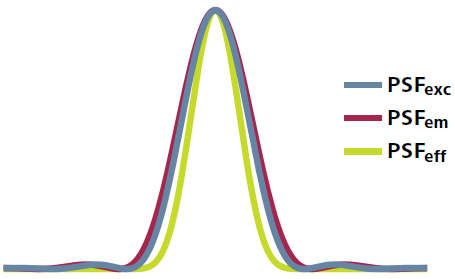
\includegraphics[width=0.9\linewidth]{blinking-1-1.png}
		\captionof{figure}{Нормированные профили ядер размытия лазера подсветки ($PSF_{exc}$), объектива ($PSF_{em}$) и микроскопа ($PSF_{eff}$)}
		\label{fig:blinking-psf}
	\end{minipage} \hfill
	\begin{minipage}{0.45\textwidth}
		\centering
		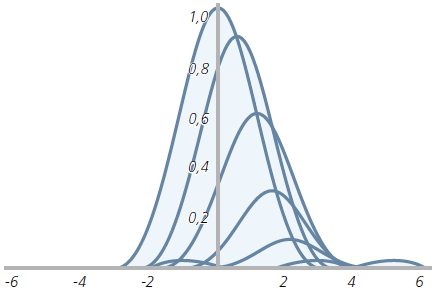
\includegraphics[width=0.9\linewidth]{blinking-1-2.png}
		\captionof{figure}{Изменение профиля ядра размытия при смещении детектора излучаемого образцов света от оптической оси}
		\label{fig:blinking-psf-displacement}
	\end{minipage}
	\hfill
\end{figure}

Изображение получается синхронно 32 детекторами: одним центральным и расположенными вокруг него тремя кольцами детекторов (Рис.~\ref{fig:blinking-airyscan}). Суммарный размер детектора Airyscan равен 1.25 диаметра диска Эйри, а размер одного элемента равен $\frac{1.25\ d_a}{6}$. Затем изображения с детекторов смещаются в сторону оптической оси с тем, чтобы положения максимумов ядер размытия детекторов совпали. Этот процесс называется переназначением пикселей (англ.~pixel reassignment)~\cite{sheppard2013superresolution}. Величина смещения $v$ изображения с одного детектора к центру определяется по формулам:

\begin{subequations}
	\begin{align}
		&v=-\frac{1}{1+\beta}\cdot\ \frac{1.25\ d_a}{6}\cdot v_d,  \nonumber \\
		&\beta=\frac{\lambda_{em}}{\lambda_{exc}},  \nonumber
	\end{align}
\end{subequations}

\noindent где $v_d$ "--- относительное смещение детектора $d$ от оптической оси в размерах детектора, $\lambda_{em}$ и $\lambda_{exc}$ "--- длины волн излучённого света и подсветки. После этого изображения суммируются, образуя изображение с более узким ядром размытия (Рис.~\ref{fig:blinking-psf-comparison}) и повышенным отношением уровня сигнала к шуму.

\begin{figure}[ht]
	\centering
	\hfill
	\begin{minipage}{0.45\textwidth}
		\centering
		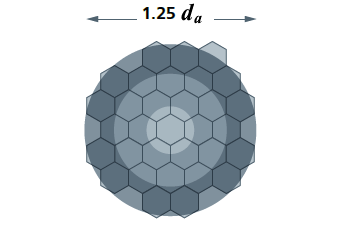
\includegraphics[width=\linewidth]{blinking-1-3-ru.png}
		\captionof{figure}{Схема детектора Airyscan. Сенсоры расположены в центрах правильных шестиугольников}
		\label{fig:blinking-airyscan}
	\end{minipage} \hfill
	\begin{minipage}{0.45\textwidth}
		\centering
		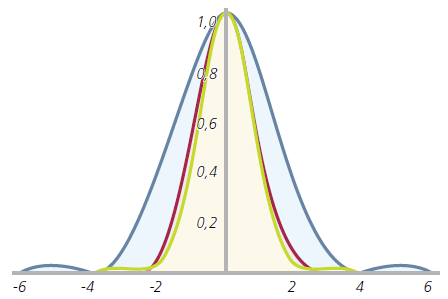
\includegraphics[width=\linewidth]{blinking-1-4.png}
		\captionof{figure}{Нормированные профили ядер размытия обычного широкопольного (синий), конфокального сканирующего (красный) микроскопов и микроскопа с детектором Airyscan (зелёный)}
		\label{fig:blinking-psf-comparison}
	\end{minipage}
	\hfill
\end{figure}

За счёт такого подхода достигается резкость конфокальных сканирующих микроскопов одновременно с высоким уровнем сигнала обычных широкопольных микроскопов, что позволяет делать длинные серии снимков с высокой частотой кадров. Примеры ядер размытия для центрального элемента и элементов каждого из колец Airyscan представлены на Рис.~\ref{fig:blinking-airyscan-psf-samples}.

\begin{figure}[ht]
	\centerfloat{
		\hfill
		\subcaptionbox[List-of-Figures entry]{Центр}{%
			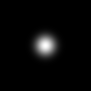
\includegraphics[width=0.2\textwidth]{blinking-1-5a.png}}
		\hfill
		\subcaptionbox{Внутреннее кольцо}{%
			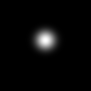
\includegraphics[width=0.2\textwidth]{blinking-1-5b.png}}
		\hfill
		\subcaptionbox{Среднее кольцо}{%
			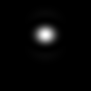
\includegraphics[width=0.2\textwidth]{blinking-1-5c.png}}
		\hfill
		\subcaptionbox{Внешнее кольцо}{%
		
\includegraphics[width=0.2\textwidth]{blinking-1-5d.png}}
		\hfill
	}
	\caption{Нормированные по яркости ядра размытия для элементов из разных слоёв детектора Airyscan}
	\label{fig:blinking-airyscan-psf-samples}
\end{figure}

\section{Рассматриваемые методы}

В данном параграфе рассматривается ряд современных методов повышения разрешения и резкости флуоресцентных изображений, полученных с использованием мигающих красителей. Далее следует описание их базовых принципов.

\subsection{Визуализация оптических флуктуаций сверхвысокого разрешения (SOFI)}

Метод SOFI (super"=resolution optical fluctuation imaging)~\cite{dertinger2009fast,dertinger2010achieving} основан на рассмотрении интенсивностей излучения молекул флуорофора как независимых случайных величин и для получения резкого изображения повышенного разрешения использует полуинварианты (англ.~cumulants) "--- коэффициенты разложения в степенной ряд логарифма характеристической функции случайной величины, которые также могут быть выражены через моменты этой случайной величины (см.~\cite{75086, малахов1978кумулянтный}).

В рамках этого подхода рассматриваются $N$ независимо мигающих флуорофоров, находящихся в позициях $\mathbf{r}_k$. Их яркости меняются со временем по закону $\varepsilon_k\cdot s_k(t)$, а итоговая интенсивность в позиции $r$ задаётся следующим образом:

\begin{equation}
	\sum_{k=1}^{N}{\delta(\mathbf{r}-\mathbf{r}_k)\cdot\varepsilon_k\cdot s_k(t)}, \quad \delta\left(\mathbf{r}-\mathbf{r}_k\right)=
	\begin{cases}
		1,\ \mathbf{r}=\mathbf{r}_k, \\
		0,\ \mathbf{r}\neq\mathbf{r}_k,
	\end{cases} \nonumber
\end{equation}	

\noindent где $\varepsilon_k$ "--- постоянная яркость молекулы красителя, а $s_k(t)$ "--- зависящая от времени функция.

Считая, что позиции молекул флуорофора не меняются со временем, а ядро размытия изображения $U(\mathbf{r})$ одинаково для всех участков изображения, интенсивность $F(\mathbf{r},t)$ в позиции $r$ в момент времени $t$ можно записать в следующем виде:

\begin{equation}
	F\left(\mathbf{r},t\right)=\sum_{k=1}^{N}{U(\mathbf{r}-\mathbf{r}_k)\cdot\varepsilon_k\cdot s_k(t)}. \nonumber
\end{equation}

Изменение интенсивности также может быть выражено как флуктуации с нулевым математическим ожиданием:

\begin{align*}
	\delta F\left(\mathbf{r},t\right) &= F\left(\mathbf{r},t\right)-\langle F\left(\mathbf{r},t\right) \rangle_t = \\
	&= \sum_{k} {U\left(\mathbf{r} - \mathbf{r}_k\right) \cdot \varepsilon_k \cdot \left[ s_k\left(t\right)- \langle s_k\left(t\right) \rangle_t \right]} = \\
	&= \sum_{k} {U\left(\mathbf{r} - \mathbf{r}_k\right) \cdot \varepsilon_k \cdot \delta s_k \left(t\right)},
\end{align*}

\noindent где $\langle \ldots \rangle_t$ означает усреднение по времени. Тогда результат работы алгоритма SOFI 2"~порядка определяется значением автокорреляционной функции изменения интенсивности $\delta F\left(\mathbf{r},t\right)$ и задаётся формулой:

\begin{align*}
	G_2\left(\mathbf{r},\tau\right) &= \langle \delta F\left(\mathbf{r},t+\tau\right)\cdot\delta F\left(\mathbf{r},t\right) \rangle_t = \\
	&= \sum_{j,k} {U\left(\mathbf{r}-\mathbf{r}_j\right)U\left(\mathbf{r}-\mathbf{r}_k\right)\cdot\varepsilon_j\cdot\varepsilon_k\cdot \langle \delta s_j\left(t+\tau\right)\delta s_k\left(t\right) \rangle_t} = \\
	&= \sum_{k} {U^2\left(\mathbf{r}-\mathbf{r}_k\right)\cdot\varepsilon_k^2\cdot \langle \delta s_k\left(t+\tau\right)\delta s_k\left(t\right) \rangle_t}.
\end{align*}

Последний переход обусловлен независимостью сигналов от молекул красителя из разных участков образца, перекрёстные члены суммы принимают нулевые значения для всех $\mathbf{r}$ и $\tau$.

Как видно из последнего уравнения, автокорреляционная функция имеет вид свёртки некоторого резкого изображения, задаваемого формулой $\sum_{k=1}^{N} {\delta(\mathbf{r}-\mathbf{r}_k)\cdot\varepsilon_k^2\cdot \langle \delta s_k\left(t+\tau\right)\delta s_k\left(t\right) \rangle_t}$, с квадратом исходного ядра размытия. Благодаря тому, что полная ширина на полувысоте (англ.~full width at half maximum, FWHM) возведённого в степень $\alpha>1$ ядра меньше, чем у исходного ядра, результат работы алгоритма SOFI обладает более высокой резкостью, чем необработанное изображение, а также позволяет достичь лучшего результата при дальнейшем восстановлении размытого изображения из-за усиленных высоких частот в спектре изображения. В частности, в случае гауссовского размытия квадрат ядра размытия в $\sqrt{2}$ раз уже самого ядра.

Можно заметить, что при $\tau=0$ значение $G_2\left(\mathbf{r},\tau\right)$ совпадает с полуинвариантом второго порядка, который равен дисперсии величины $\delta F\left(\mathbf{r},t\right)$.

Для порядков SOFI выше второго используется не автокорреляционная функция, а полуинварианты соответствующих порядков, так как в противном случае перекрёстные члены в сумме остаются.

Хотя теоретического ограничения на степень повышения резкости нет, на практике используются полуинварианты порядков не выше четвёртого из-за роста влияния шума на результат с ростом порядка полуинварианта. А поскольку результат преобразования содержит не яркость молекул, а значения, зависящие от колебания яркости, которые могут быть в том числе равными нулю или меньше него, то только полуинвариант второго порядка (дисперсия яркости) даёт наиболее устойчивый результат с минимальной потерей данных и деталей изображения. Это и обусловило выбор второго порядка SOFI для проведения сравнения методов.

При замене полуинвариантов на смешанные полуинварианты (англ.~joint cumulants) "--- коэффициенты разложения в степенной ряд логарифма характеристической функции случайного вектора, составленного из нескольких случайных величин (см.~\cite{малахов1978кумулянтный}) "--- получившийся алгоритм XC"~SOFI $n$"~го порядка~\cite{dertinger2010achieving}, помимо повышения резкости, обеспечивает и повышение разрешения в $n$ раз. В этом случае в преобразовании участвует несколько соседних пикселей изображения. В частности, для второго порядка получаем следующее выражение:

\begin{align*}
	&{XC}_2\left(\mathbf{r}_1,\mathbf{r}_2,\tau_1,\tau_2\right) = \\
	&= \sum_{i=1}^{N} {U\left(\mathbf{r}_1-\mathbf{r}_i\right)U\left(\mathbf{r}_2-\mathbf{r}_i\right)\cdot\varepsilon_k^2\cdot \langle \delta s_i\left(t+\tau_1\right)\delta s_i\left(t+\tau_2\right) \rangle_t} = \\
	&= U\left(\frac{\mathbf{r}_1-\mathbf{r}_2}{\sqrt2}\right) \sum_{i=1}^{N} {U^2\left(\frac{\mathbf{r}_1+\mathbf{r}_2}{2}-\mathbf{r}_i\right)\cdot\varepsilon_i^2\cdot \langle \delta s_i\left(t+\tau_1\right)\delta s_i\left(t+\tau_2\right) \rangle_t}.
\end{align*}

Отсюда видно, что:
\begin{enumerate}[beginpenalty=10000]
	\item Позиция результирующего пикселя лежит между двумя пикселями, участвующими в преобразовании.
	\item Результирующий пиксель имеет дополнительный множитель $U\left(\frac{\mathbf{r}_1-\mathbf{r}_2}{\sqrt2}\right)$, поэтому необходимо произвести перевзвешивание результирующего изображения для приведения уровня яркости разных групп пикселей к одному. При неизвестном ядре размытия это можно сделать, например, нормировав яркости пикселей каждой группы на среднее отклонение или математическое ожидание их яркостей.
\end{enumerate}

Для более высоких порядков формула приобретает вид:	

\begin{equation*}
	\begin{multlined}
		{XC}_n\left(\mathbf{r}_1,{\ldots,\mathbf{r}}_n,\tau_1,{\ldots,\tau}_n \right) = \\
		= \prod_{j<l}^{n}{U\left(\frac{\mathbf{r}_j-\mathbf{r}_l}{\sqrt n}\right)} \cdot \sum_{i=1}^{N}{U^n\left(\frac{\sum_{k}^{n}\mathbf{r}_k}{n}-\mathbf{r}_i \right)\cdot\varepsilon_i^n\cdot w_i(\tau_1,\ldots,\tau_n)},
	\end{multlined}
\end{equation*}

\noindent где $w_i$ "--- смешанный полуинвариант функций $s_i(t)$ порядка $n$.

\subsection{Алгоритм классификации множественных сигналов для флуоресцентной микроскопии сверхвысокого разрешения MUSICAL}

Метод повышения разрешения и резкости изображений MUSICAL (Multiple signal classification algorithm for super-resolution fluorescence microscopy)~\cite{agarwal2016multiple} основан на методе разделения нескольких сигналов MUSIC~\cite{schmidt1986multiple}.

В рамках этого метода интенсивность $n$"~го пикселя $k$"~го кадра ($1\le k\le K$, где $K$ "--- общее число изображений в обрабатываемой серии) задаётся формулой

\begin{equation}
	I_k\left({\vec{r}}_n\right)=\int_{y_n-\frac{w}{2}}^{y_n+\frac{w}{2}}\int_{x_n-\frac{w}{2}}^{x_n+\frac{w}{2}}\sum_{m=1}^{M}{G\left({\vec{r}}_n,{\vec{r}}_m^{\,\prime}\right)\ s_m\left(k\right)\ dx\ dy}\approx\sum_{m=1}^{M}{w^{2\ }G\left({\vec{r}}_n,{\vec{r}}_m^{\,\prime}\right){\ s}_m\left(k\right)}, \nonumber
\end{equation}	

\noindent где ${\vec{r}}_n=(x_n,y_n)$ "--- позиция $n$"~го пикселя в плоскости изображения, $w$ "--- длина его стороны, ${\vec{r}}_m^{\,\prime}$ "--- позиция $m$"~го флуорофора в плоскости образца, $s_m\left(k\right)\geq0$ "--- суммарное излучение от $m$"~го флуорофора за время выдержки $k$"~го кадра (при этом $\exists k: {s}_m\left(k\right)>0$), а $G\left(\vec{r},{\vec{r}}^{\,\prime}\right)\ \geq\ 0$ "--- функция, определяющая ядро размытия, отображающая интенсивность излучения из точки ${\vec{r}}^{\,\prime}$ в плоскости образца в точку $\vec{r}$ в плоскости изображения.

Таким образом, интенсивности всех пикселей $k$"~го изображения могут быть записаны в виде матричного уравнения: ${\overline{I}}_k=\mathbf{G}{\overline{s}}_k$, где

\begin{align*}
	&{\overline{I}}_k=\left[
		\begin{array}{cccc}
			I_k\left({\vec{r}}_1\right) & I_k\left({\vec{r}}_2\right) & \cdots & I_k\left({\vec{r}}_N\right)
		\end{array}
	\right]^\mathrm{T}, \\
	&\mathbf{G}=w^2 \left[
		\begin{array}{cccc}
			\overline{G}\left({\vec{r}}_1^{\,\prime}\right) & \overline{G}\left({\vec{r}}_2^{\,\prime}\right) & \cdots & \overline{G}\left({\vec{r}}_M^{\,\prime}\right)
		\end{array}
	\right], \\
	&\overline{G}\left({\vec{r}}^{\,\prime}\right)=\left[
		\begin{array}{cccc}
			G\left({\vec{r}}_1,{\vec{r}}^{\,\prime}\right) & G\left({\vec{r}}_2,{\vec{r}}^{\,\prime}\right) & \cdots & G\left({\vec{r}}_N,{\vec{r}}^{\,\prime}\right)
		\end{array}
	\right]^\mathrm{T}, \\
	&{\overline{s}}_k=\left[
		\begin{array}{cccc}
			s_1\left(k\right) & s_2\left(k\right) & \cdots & s_M\left(k\right)
		\end{array}
	\right]^\mathrm{T}.
\end{align*}

Полный набор изображений может быть записан матрицей

\begin{equation*}
	\mathbf{I} = \left[
		\begin{array}{cccc}
			{\overline{I}}_1 & {\overline{I}}_2 & \cdots & {\overline{I}}_K
		\end{array}
	\right] = \mathbf{G} \cdot \left[
		\begin{array}{cccc}
			{\overline{s}}_1 & {\overline{s}}_2 & \cdots & {\overline{s}}_K
		\end{array}
	\right].
\end{equation*}

Отсюда видно, что каждый столбец матрицы $\mathbf{I}$ "--- это линейная комбинация столбцов матрицы $\mathbf{G}$, а пространство столбцов матрицы $\mathbf{I}$, являющееся линейной оболочкой полученных изображений, определяется пространством столбцов матрицы $\mathbf{I}$. Одновременно с этим пространство столбцов матрицы $\mathbf{I}$ задаётся левыми сингулярными векторами из сингулярного разложения этой матрицы, у которых соответствующие им сингулярные числа не равны нулю: $\left\{{\overline{u}}_{\sigma_i\neq0}\right\}$.

Если $\mathbf{I}$ "--- матрица неполного ранга, то существует линейное пространство векторов $\left\{{\overline{u}}_{\sigma_i=0}\right\}$, ортогональное пространству столбцов матрицы $\mathbf{I}$, и выполняется $\overline{G}\left({\vec{r}}_m^{\,\prime}\right) \cdot {\overline{u}}_{\sigma_i=0}=0$ для всех $m$. При условии, что флуорофоры мигают независимо, одному элементу из $\left\{\overline{G}\left({\vec{r}}_m^{\,\prime}\right); m=\overline{1;M}\right\}$ соответствует один и только один элемент из $\left\{{\overline{u}}_{\sigma_i\neq0}\right\}$. Поэтому вектора $\overline{G}\left({\vec{r}}^{\,\prime}\right)$ для позиций ${\vec{r}}^{\,\prime} \notin \left\{{\vec{r}}_m^{\,\prime},\ m=\overline{1;M}\right\}$ имеют ненулевую проекцию на линейное пространство векторов $\left\{{\overline{u}}_{\sigma_i=0}\right\}$.

В случае полного ранга выбирается некоторый порог $\sigma_0$ и за базис пространства столбцов матрицы берётся множество $\left\{{\overline{u}}_{\sigma_i\geq\sigma_0}\right\}$, а за базис ортогонального сигналу пространства "--- $\left\{{\overline{u}}_{\sigma_i<\sigma_0}\right\}$. Обусловлен такой подход тем, что разные вектора ${\overline{u}}_{\sigma_i}$ соответствуют разным структурным деталям изображений, соответствующие им $\sigma_i^2$ определяют энергию (силу) этих векторов, а вектора с низкой энергией могут быть сильно искажены шумом и не могут считаться надёжными при восстановлении изображения высокого разрешения.

Для проверки условий принадлежности вектора $\overline{G}\left({\vec{r}}^{\,\prime}\right)$ к $\left\{\overline{G}\left({\vec{r}}_m^{\,\prime}\right); m=\overline{1;M}\right\}$ в MUSICAL используется индикаторная функция с параметром $\alpha$, отвечающим за контраст:

\begin{align*}
	&f\left({\vec{r}}_{test}^{\,\prime}\right) = \left(\frac{d_{PR}\left({\vec{r}}_{test}^{\,\prime}\right)} {d_{PN}\left({\vec{r}}_{test}^{\,\prime}\right)}\right)^\alpha, \\
	&d_{PR}\left({\vec{r}}_{test}^{\,\prime}\right) = \sqrt{\sum_{\sigma_i\geq\sigma_0}{\lVert \overline{G}\left({\vec{r}}_{test}^{\,\prime}\right)\cdot{\overline{u}}_i \rVert}^2}, \\
	&d_{PN}\left({\vec{r}}_{test}^{\,\prime}\right) = \sqrt{\sum_{\sigma_i<\sigma_0}{\lVert \overline{G}\left({\vec{r}}_{test}^{\,\prime}\right)\cdot{\overline{u}}_i \rVert}^2}.
\end{align*}

Значения такой индикаторной функции будут тем больше, чем ближе точка ${\vec{r}}^{\,\prime}$ к позиции одного из $m$ флуорофоров. Посчитав значения этой функции для всех пикселей изображения высокого разрешения, можно построить своего рода карту расположения молекул флуорофоров.

Для ускорения работы алгоритма и устойчивости определения базиса пространства сигнала алгоритм MUSICAL обрабатывает изображение не целиком, а с использованием скользящего окна, сопоставимого по размеру с диаметром ядра размытия, с дальнейшим усреднением значений индикаторной функции в областях перекрытия окон.

\subsection{Байесовский анализ мигания и выгорания 3B}

Ещё одним рассмотренным методом является метод локализации молекул флуорофора с помощью байесовского алгоритма локализационной микроскопии~\cite{cox2012bayesian}. Метод использует скрытую марковскую модель для представления переходов флуорофора между тремя состояниями (излучает, не излучает, разрушен) и делает вывод о присутствии флуорофора в точке на основе отношения вероятности его присутствия (событие $\mathcal{F}$) в этой точке при учёте наблюдаемых данных $D$ к вероятности его отсутствия (событие $\mathcal{N}$) при тех же данных: $\frac{p\left(\mathcal{F}\middle| D\right)}{p\left(\mathcal{N}\right|D)} = \frac{p\left(D\middle|\mathcal{F}\right)p\left(\mathcal{F}\right)} {p\left(D\middle|\mathcal{N}\right)p\left(\mathcal{N}\right)}$. Так как $p\left(\mathcal{F}\right)$ и $p\left(\mathcal{N}\right)$ постоянные, то оценить нужно только вероятности $p\left(D\middle|\mathcal{F}\right)$ и $p\left(D\middle|\mathcal{N}\right)$. Последнее "--- это вероятность наблюдения данных при учёте наличия в них только шума известной модели (например, шума с нормальным распределением). Первая величина вычисляется следующим образом:

\begin{equation*}
	p\left(D\middle|\mathcal{F}\right)=\int_{a\in\mathbb{R}^4}\int_{b\in\mathbb{Z}_3^N}{p\left(D,a,b\middle|\mathcal{F}\right)\ db\ da},
\end{equation*}

\noindent где $a$ "--- 4 параметра каждого флуорофора (координаты в плоскости изображения, яркость и размер), а $b$ "--- набор состояний флуорофора в каждом кадре. Вероятность $p\left(D,a,b\middle|\mathcal{F}\right)$ равна произведению вероятности получения наблюдаемых данных при условии наличия флуорофора в рассматриваемой точке на априорные вероятности параметров $a$ и $b$. Априорные вероятности координат флуорофоров заданы равномерным распределением на рассматриваемой области изображения и нулём вне этой области. Размер изображения флуорофора имеет логнормальное априорное распределение с параметрами $\sigma=0.1$ и $\mu$ таким, чтобы мода распределения имела значение полной ширины на полувысоте заданного ядра размытия. Априорное распределение яркости флуорофора тоже логнормальное, с параметрами $\sigma=3$ и $\mu=1$. Априорное распределение состояния флуорофора в первом кадре задано так, чтобы вероятности состояний <<излучает>> и <<не излучает>> были равновероятными, а событие <<флуорофор разрушен>> "--- невозможным. Дальнейшие априорные вероятности вычисляются с использованием скрытой марковской модели в зависимости от предыдущих состояний.

С учётом всех $M$ молекул флуорофора уравнение приобретает вид:

\begin{equation*}
	p\left(D\middle|\mathcal{F}_M\right)=\int_{a\in\mathbb{R}^{4 \cdot M}}\int_{b\in\mathbb{Z}_3^{N \cdot M}}{p\left(D,a,b\middle|\mathcal{F}_M\right)\ db\ da}.
\end{equation*}	

Из-за большого объёма вычислений в случае многих молекул интегрирование по $a$ проводится приближённо методом Лапласа, а интеграл по $b$ оценивается с помощью генерации выборки $\left\{b_i\right\}_{i=1\ }^n$ методом Монте"=Карло по схеме марковской цепи и вычисления суммы

\begin{equation*}
	p\left(D\middle|\mathcal{F}_M\right)=\int_{a\in\mathbb{R}^{4 \cdot M}}\int_{b\in\mathbb{Z}_3^{N \cdot M}}{p\left(D,a,b\middle|\mathcal{F}_M\right)\ db\ da} \approx \frac{1}{n}\int_{a\in\mathbb{R}^{4 \cdot M}}{\sum_{i=1}^{n}{p\left(D,a,b_i\middle|\mathcal{F}_M\right)}}.
\end{equation*}

\section{Численный метод повышения разрешения и резкости изображений}

В ходе выполнения исследования нами был разработан и реализован итерационный алгоритм повышения резкости и разрешения изображений на основе байесовского подхода.

В основе метода лежит предположение о том, что интенсивности пикселей резкого изображения можно рассмотреть как независимые случайные величины, а серию резких изображений "--- как результат серии наблюдений этих случайных величин. Влияние дифракции представлено свёрткой резкого изображения с одним и тем же ядром для всех пикселей и всех кадров, а полученные размытые снимки содержат высокочастотный шум.

В рамках предлагаемого подхода размытые зашумлённые изображения серии рассматриваются как наблюдаемые переменные, соответствующие им исходные резкие изображения "--- как скрытые, а среднее значение и дисперсия интенсивности каждого пикселя исходной серии изображений "--- как неизвестные параметры распределения интенсивности этого пикселя. Затем эти параметры распределений интенсивностей пикселей вычисляются с помощью байесовского алгоритма. При этом полученные дисперсии интенсивностей можно трактовать как высококонтрастную карту объектов с изменяющейся яркостью, на которой подсвеченный мигающим флуорофором образец будет присутствовать, а постоянный фон "--- нет.

На вход разработанного алгоритма поступает набор размытых и зашумлённых изображений $Y=\left\{y^t\right\}_{t=1}^T$, $y^t\in\mathbb{R}^l$, ему соответствует неизвестный набор резких изображений высокого разрешения $X=\left\{x^t\right\}_{t=1}^T$, $x^t\in\mathbb{R}^n$. Благодаря природе шума, его можно моделировать случайным процессом с нормальным распределением~\cite{gadsden1965some}. Поэтому в данном пункте считается, что $y^t \sim N({Kx}^t,\Theta^{-1})$, где $K\in\mathbb{R}^{l \times n}$ "--- оператор свёртки и понижения разрешения (имеет вид матрицы Тёплица с элементами ядра размытия на диагоналях, умноженной на матрицу понижения разрешения слева), а $\Theta\in\mathbb{R}^{n \times n}$ "--- обратная ковариационная матрица шума, диагональная из-за попиксельной независимости шума. Предполагается, что вследствие малого размера молекул флуорофора в каждом пикселе изображения может находиться достаточно много независимо мигающих молекул, чтобы можно было приблизить распределение суммарной яркости точки нормальным распределением: $x^t \sim N(\mu,\Lambda^{-1})$, где $\mu\in\mathbb{R}^n$ "--- средняя по всем кадрам яркость объекта, а $\Lambda\in\mathbb{R}^{n \times n}$ "--- обратная ковариационная матрица мерцания объекта.

Финальным результатом работы алгоритма являются оценки средней яркости образца $\mu$ и диагонали ковариационной матрицы $\Lambda^{-1}$, квадратные корни элементов которой является стандартными отклонениями яркостей точек резких изображений.

Рассматривая $X$, $\mu$ и $\Lambda$ как скрытые переменные, можно записать их совместное апостериорное распределение:

\begin{equation*}
	p\left(X,\mu,\Lambda\middle|Y,\Theta\right)=\frac{p\left(Y\middle|X,\Theta\right)p\left(X\middle|\mu,\Lambda\right)p\left(\mu\right)p\left(\Lambda\right)}{p\left(Y\middle|\Theta\right)}.
\end{equation*}

Для нахождения распределений $\mu$ и $\Lambda$ и матрицы $\Theta$ максимизируется правдоподобие набора кадров:

\begin{equation*}
	p\left(Y\middle|\Theta\right) \rightarrow \max_{p \left( X, \mu, \Lambda \middle| Y,\Theta \right),\Theta}
\end{equation*}
с помощью EM"~алгоритма~\cite{477e7e2b-4ded-3369-981e-9b40850a2701} с использованием аппроксимации среднего поля (англ.~mean field approximation)~\cite{bishop2006pattern}.

Апостериорное совместное распределение аппроксимируется факторизуемой плотностью вероятности:

\begin{equation*}
	p\left(X,\mu,\Lambda\middle|Y,\Theta\right)\approx q\left(X,\mu,\Lambda\right)=\prod_{t=1}^{T}{q_{1,t}\left(x^t\right)\cdot\ q_2\left(\mu\right)\cdot q_3\left(\Lambda\right)},
\end{equation*}

\noindent где в качестве множителей $q_{1,t}\left(x^t\right)$ и $q_2\left(\mu\right)$ используются нормальные распределения, а для $q_3\left(\Lambda\right)$ "--- распределение Уишарта.

Априорные распределения $p\left(\mu\right)$ и $p\left(\Lambda\right)$ в рамках исследования задаются следующим образом:

\begin{align*}
	&\mu \sim N\left(m_0,\ \eta_0^{-1}I_n\right), \\
	&\Lambda \sim W\left(W_0,\nu_0\right)=\frac{1}{C}\left|\Lambda\right|^\frac{\nu_0-n-1}{2}\exp{\left(-\frac{1}{2}tr\left[W_0^{-1}\Lambda\right]\right)},
\end{align*}

\noindent где $W(\cdots)$ "--- распределение Уишарта, $I_n$ "--- единичная матрица, $m_0\in\mathbb{R}^n$, $\eta_0,\ \nu_0\in\mathbb{R}$ и $W_0\in\mathbb{R}^{n \times n}$ "--- параметры метода, а $C$ "--- нормировочная константа. Вид распределений выбран в том числе с тем, чтобы получить аналитическое решение одного из шагов алгоритма оптимизации, однако в то же время для $\mu$ после преобразований это эквивалентно добавлению стабилизатора вида $\frac{\eta_0}{2} \lVert x - m_0 \rVert^2$ на E"~шаге EM"~алгоритма.

При таких условиях совместная плотность вероятности наблюдаемых размытых зашумлённых изображений и соответствующих им <<скрытых>> резких изображений имеет следующий вид:

\begin{align*}
	p\left(Y,X,\mu,\Lambda \middle| \Theta\right) &= \prod_{t=1}^{T} \left( \frac{\lvert\Theta\rvert \cdot \lvert\Lambda\rvert}{{\left(2\pi\right)}^{l+n}} \right)^\frac{1}{2} \exp\left(
	\begin{aligned}
		&-\frac{1}{2}\left(y^t-Kx^t\right)^\mathrm{T} \Theta \left(y^t-Kx^t\right) - \\
		&-\frac{1}{2}\left(x^t-\mu\right)^\mathrm{T} \Lambda \left(x^t-\mu\right)
	\end{aligned}
	\right) \cdot \\
	&\cdot \left(\frac{\eta_0}{2\pi}\right)^\frac{n}{2} \exp \left(-\frac{1}{2}\left(\mu-m_0\right)^\mathrm{T} \eta_0 I_n \left(\mu-m_0\right)\right) \cdot \\
	&\cdot \frac{1}{C}\lvert\Lambda\rvert^\frac{\nu_0-n-1}{2}\exp{\left(-\frac{1}{2}tr\left[W_0^{-1}\Lambda\right]\right)}.
\end{align*}

Тогда параметры распределений $X$, $\mu$ и $\Lambda$ и матрица $\Theta$ находятся итерационным алгоритмом, который на каждом шаге пересчитывает их по очереди в соответствии с уравнениями:

\begin{align*}
	&\log{q_{1,k}\left(x^k\right)}=\mathbb{E}_{\left\{x^{t \backslash k}\right\},\mu,\Lambda}\log{p\left(Y,X,\mu,\Lambda\mid\Theta\right)}+C_{1,k}, \\
	&\log{q_2\left(\mu\right)}=\mathbb{E}_{\left\{x^t\right\},\Lambda}\log{p\left(Y,X,\mu,\Lambda\mid\Theta\right)}+C_2, \\
	&\log{q_3\left(\Lambda\right)}=\mathbb{E}_{\left\{x^t\right\},\mu}\log{p\left(Y,X,\mu,\Lambda\mid\Theta\right)}+C_3, \\
	&\Theta=\arg{\max_\Theta{\mathbb{E}_{\left\{x^t\right\},\mu,\Lambda}\log{p\left(Y,X,\mu,\Lambda\mid\Theta\right)}}},
\end{align*}

\noindent где $\left\{C_{1,k}\right\}_{k=1}^T$, $C_2$ и $C_3$ "--- нормировочные константы.

Итоговый алгоритм выглядит следующим образом:

\begin{enumerate}[beginpenalty=10000]
	\item Задаются начальные приближения некоторых параметров искомых распределений $\mu$ и $\Lambda$ и матрицу $\Theta$: $\mathbb{E}\mu \gets \mathbb{E}y^t$, $\mathbb{E}\Lambda \gets diag\left(D\left( y^t \right)\right)$, $\Theta \gets \theta I_l$, где $\theta$ "--- эмпирическая оценка шума, выполненная в пустой области изображения.
	
	\item В течение $R$ итераций происходит обновление параметров искомых распределений:
	
	\begin{align*}
		&q_{1,t}\left(x^t\right):\ \Sigma_{x^t} \gets \left(K^\mathrm{T} \Theta K+\mathbb{E}\Lambda\right)^{-1},\ \ \mathbb{E}x^t \gets \Sigma_{x^t} \cdot \left(K^\mathrm{T} \Theta y^t+\mathbb{E}\Lambda\cdot\mathbb{E}\mu\right); \\
		&q_2\left(\mu\right):\ \Sigma_\mu \gets \left(T\cdot\mathbb{E}\Lambda+\eta_0 I_n\right)^{-1},\ \ \mathbb{E}\mu \gets \Sigma_\mu \cdot \left(\mathbb{E}\Lambda\cdot\sum_{t=1}^{T}{\mathbb{E}x^t}+\eta_0 I_nm_0\right); \\
		&q_3\left(\Lambda\right):\ W\left(W^\prime,v^\prime\right),\ v^\prime \gets v_0+T, \\
		&W^\prime \gets \left(W_0^{-1}+\sum_{t=1}^{T}\left[
		\begin{aligned}
			&\Sigma_{x^t} + \mathbb{E}x^t\left(\mathbb{E}x^t\right)^\mathrm{T} - \mathbb{E}x^t\left(\mathbb{E}\mu\right)^\mathrm{T} - \\
			&- \mathbb{E}\mu\left(\mathbb{E}x^t\right)^\mathrm{T} + \Sigma_\mu + \mathbb{E}\mu\left(\mathbb{E}\mu\right)^\mathrm{T}
		\end{aligned}
		\right]\right)^{-1}, \\
		&\mathbb{E}\Lambda \gets v^\prime W^\prime; \\
		%	&\Theta \gets \left(\frac{1}{T}\sum_{t=1}^{T}\left[\left(K\mathbb{E}x^t-y^t\right)\left(K\mathbb{E}x^t-y^t\right)^\mathrm{T}+K\Sigma_{x^t}K^\mathrm{T}\right]\right)^{-1}. \\
		&\Theta_{ii} \gets \left(\frac{1}{T}\sum_{t=1}^{T}\left[\left(\left(K\mathbb{E}x^t - y^t\right)_i\right)^2 + \left(K\Sigma_{x^t}K^\mathrm{T}\right)_{ii}\right]\right)^{-1}.
	\end{align*}
	
\end{enumerate}

%\begin{align*}
%	&q_{1,t}\left(x^t\right):\ \Sigma_{x^t}=\left(K^\mathrm{T} \Theta K+\mathbb{E}\Lambda\right)^{-1},\ \mathbb{E}x^t=\Sigma_{x^t} \cdot \left(K^\mathrm{T} \Theta y^t+\mathbb{E}\Lambda\cdot\mathbb{E}\mu\right); \\
%	&q_2\left(\mu\right):\ \Sigma_\mu=\left(T\cdot\mathbb{E}\Lambda+\eta_0 I_n\right)^{-1},\ \mathbb{E}\mu=\Sigma_\mu \cdot \left(\mathbb{E}\Lambda\cdot\sum_{t=1}^{T}{\mathbb{E}x^t}+\eta_0 I_nm_0\right); \\
%	&q_3\left(\Lambda\right):\ W\left(W^\prime,v^\prime\right),\ v^\prime=v_0+T \\
%	&W^\prime=\left(W_0^{-1}+\sum_{t=1}^{T}\left[
%	\begin{aligned}
%		&\Sigma_{x^t} + \mathbb{E}x^t\left(\mathbb{E}x^t\right)^\mathrm{T} - \mathbb{E}x^t\left(\mathbb{E}\mu\right)^\mathrm{T} - \\
%		&- \mathbb{E}\mu\left(\mathbb{E}x^t\right)^\mathrm{T} + \Sigma_\mu + \mathbb{E}\mu\left(\mathbb{E}\mu\right)^\mathrm{T}
%	\end{aligned}
%	\right]\right)^{-1}, \\
%	&\mathbb{E}\Lambda=v^\prime W^\prime; \\
%%	&\Theta=\left(\frac{1}{T}\sum_{t=1}^{T}\left[\left(K\mathbb{E}x^t-y^t\right)\left(K\mathbb{E}x^t-y^t\right)^\mathrm{T}+K\Sigma_{x^t}K^\mathrm{T}\right]\right)^{-1}. \\
%	&\Theta_{ii}=\left(\frac{1}{T}\sum_{t=1}^{T}\left[\left(\left(K\mathbb{E}x^t - y^t\right)_i\right)^2 + \left(K\Sigma_{x^t}K^\mathrm{T}\right)_{ii}\right]\right)^{-1}.
%\end{align*}

В качестве оценок средней яркости образца и карты мерцания его точек используются величины $\mathbb{E}\mu$ и $\left(\mathbb{E}\Lambda\right)^{-1}$ соответственно.

Для ускорения работы алгоритма он может быть запущен без учёта повышения разрешения, а затем полученный результат после простой интерполяции может быть использован в качестве начального приближения при нахождении изображения повышенного разрешения.

\section{Эксперименты и результаты}

В ходе исследования методы SOFI, MUSICAL и разработанный итерационный алгоритм были реализованы на языке программирования Python. Для получения результатов обработки изображений алгоритмом 3B было использовано программное обеспечение от авторов этого метода (доступно по ссылке \url{http://www.coxphysics.com/3b}).

При тестировании алгоритма SOFI для уменьшения влияния пространственно некоррелированного шума на интенсивность пикселей результирующего изображения был выбран его вариант XC"~SOFI, применяющий смешанные полуинварианты. Для каждого пикселя исходного изображения вычислялись смешанные полуинварианты второго порядка его ближайших соседних пикселей, расположенных напротив друг друга, а затем полученные величины усреднялись.

%Была проведена оптимизация алгоритма SOFI для уменьшения влияния пространственно некоррелированного шума на интенсивность пикселей изображения высокого разрешения в позициях исходных пикселей путём замены вычисления автокорреляции исходных пикселей на вычисление усреднённых смешанных полуинвариантов сигналов с пикселей вокруг исходных.

Было проведено тестирования рассматриваемых алгоритмов на искусственных и реальных данных, примеры результатов обработки представлены на Рис.~\ref{fig:blinking-results-simulation}~и~\ref{fig:blinking-results-real}. Разработанный итерационный метод был ускорен с использованием технологии Nvidia~CUDA, тестирование остальных методов проводилось на ЭВМ с четырёхядерным процессором Intel~Core~i5~6500. Среднее время работы на представленных данных составило для XC"~SOFI второго порядка вместе с дальнейшим устранением размытия "--- 2 секунды, для 3B "--- 45 минут, для разработанного итерационного метода "--- 2 минуты, для MUSICAL "--- 1 минута. Использовались значения параметров $m_0 = \left(0, \ldots,  0\right)^\mathrm{T}$, $\eta_0 = 10^{-6}$, $v_0 = 10^{-5} + n + 1$, $W_0 = 10^8 I_n$, $R=128$.

\begin{figure}[ht]
	\centerfloat{
		\hfill
		\subcaptionbox[List-of-Figures entry]{Карта молекул флуорофора}{%
			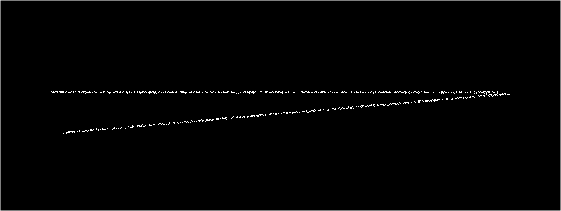
\includegraphics[width=0.3\textwidth]{blinking-1-7a.png}}
		\hfill
		\subcaptionbox{Пример одного изображения серии}{%
			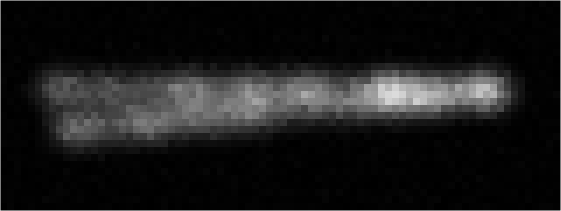
\includegraphics[width=0.3\textwidth]{blinking-1-7b.png}}
		\hfill
		\subcaptionbox{Усреднённое по времени изображение\label{fig:blinking-results-avg-sim}}{%
			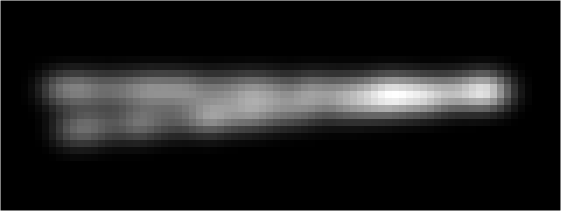
\includegraphics[width=0.3\textwidth]{blinking-1-7c.png}}
		\hfill
		\vfill
		\hfill
		\subcaptionbox{Устранение размытия на Рис.~\ref{fig:blinking-results-avg-sim} методом Люси"=Ричардсона~\cite{richardson1972bayesian}}{%
			
\includegraphics[width=0.3\textwidth]{blinking-1-7d.png}}
		\hfill
		\subcaptionbox{XC"~SOFI порядка~2\label{fig:blinking-results-sofi-2-sim}}{%
			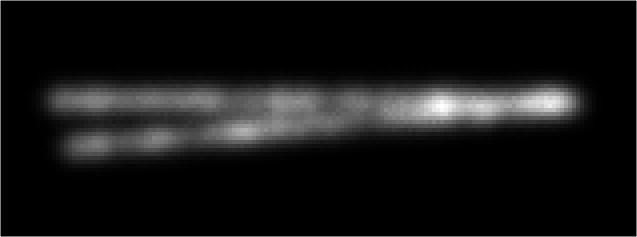
\includegraphics[width=0.3\textwidth]{blinking-1-7e.png}}
		\hfill
		\subcaptionbox{Устранение размытия на Рис.~\ref{fig:blinking-results-sofi-2-sim} методом Люси"=Ричардсона}{%
			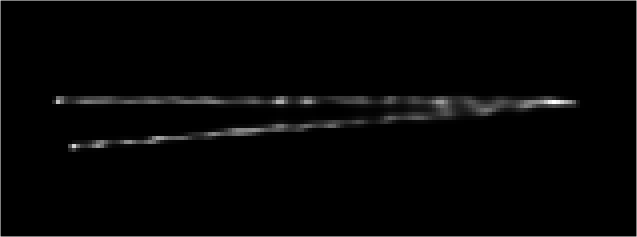
\includegraphics[width=0.3\textwidth]{blinking-1-7f.png}}
		\hfill
		\vfill
		\hfill
		\subcaptionbox{XC"~SOFI порядка~3\label{fig:blinking-results-sofi-3}}{%
			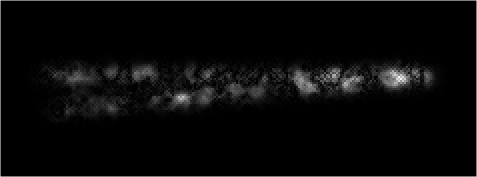
\includegraphics[width=0.3\textwidth]{blinking-1-7g.png}}
		\hfill
		\subcaptionbox{Устранение размытия на Рис.~\ref{fig:blinking-results-sofi-3} методом Люси"=Ричардсона}{%
			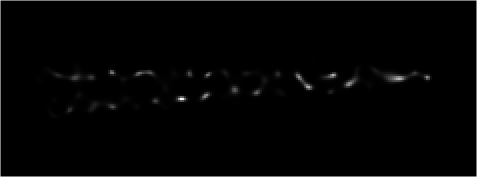
\includegraphics[width=0.3\textwidth]{blinking-1-7h.png}}
		\hfill
		\subcaptionbox{3B}{%
			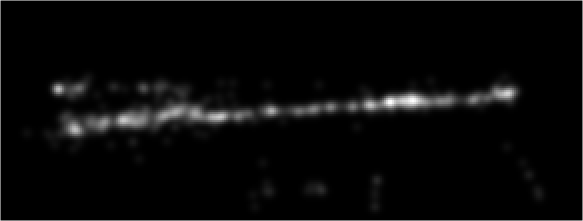
\includegraphics[width=0.3\textwidth]{blinking-1-7i.png}}
		\hfill
		\vfill
		\hfill
		\subcaptionbox{Разработанный метод, средняя яркость}{%
			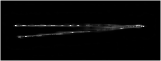
\includegraphics[width=0.3\textwidth]{blinking-1-7j.png}}
		\hfill
		\subcaptionbox{Разработанный метод, стандартные отклонения яркости}{%
			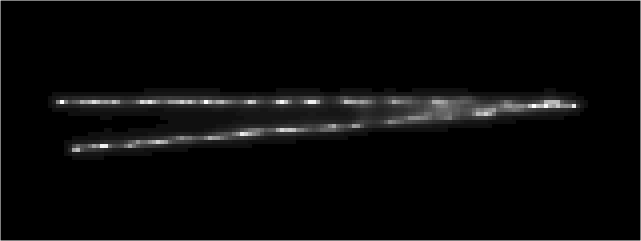
\includegraphics[width=0.3\textwidth]{blinking-1-7k.png}}
		\hfill
		\subcaptionbox{MUSICAL}{%
			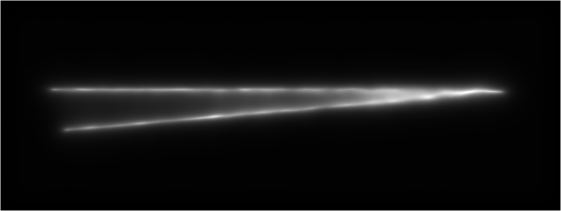
\includegraphics[width=0.3\textwidth]{blinking-1-7l.png}}
		\hfill
		\vfill
	}
	\caption{Примеры изображений из искусственного набора данных и результаты работы рассмотренных алгоритмов}
	\label{fig:blinking-results-simulation}
\end{figure}

\begin{figure}[ht]
	\centerfloat{
		\hfill
		\subcaptionbox[List-of-Figures entry]{Один кадр серии}[0.3\textwidth]{%
			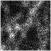
\includegraphics[width=0.2\textwidth]{blinking-1-8a.png}}
		\hfill
		\subcaptionbox{Усреднённое по времени изображение\label{fig:blinking-results-avg-real}}[0.3\textwidth]{%
			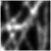
\includegraphics[width=0.2\textwidth]{blinking-1-8b.png}}
		\hfill
		\subcaptionbox{Устранение размытия на Рис.~\ref{fig:blinking-results-avg-real} методом Люси"=Ричардсона}[0.3\textwidth]{%
			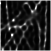
\includegraphics[width=0.2\textwidth]{blinking-1-8c.png}}
		\hfill
		\vfill
		\hfill
		\subcaptionbox{XC"~SOFI порядка~2\label{fig:blinking-results-sofi-2-real}}[0.3\textwidth]{%
			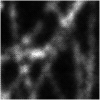
\includegraphics[width=0.2\textwidth]{blinking-1-8d.png}}
		\hfill
		\subcaptionbox{Устранение размытия на Рис.~\ref{fig:blinking-results-sofi-2-real} методом Люси-Ричардсона}[0.3\textwidth]{%
			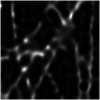
\includegraphics[width=0.2\textwidth]{blinking-1-8e.png}}
		\hfill
		\subcaptionbox{XC"~SOFI порядка~3}[0.3\textwidth]{%
			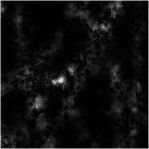
\includegraphics[width=0.2\textwidth]{blinking-1-8f.png}}
		\hfill
		\vfill
		\hfill
		\subcaptionbox{3B}[0.3\textwidth]{%
			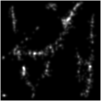
\includegraphics[width=0.2\textwidth]{blinking-1-8g.png}}
		\hfill
		\subcaptionbox{Разработанный метод, стандартные отклонения яркости}[0.3\textwidth]{%
			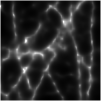
\includegraphics[width=0.2\textwidth]{blinking-1-8h.png}}
		\hfill
		\subcaptionbox{MUSICAL}[0.3\textwidth]{%
			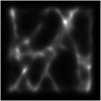
\includegraphics[width=0.2\textwidth]{blinking-1-8i.png}}
		\hfill
		\vfill
	}
	\caption{Примеры изображений из реального набора данных и результаты работы рассмотренных алгоритмов}
	\label{fig:blinking-results-real}
\end{figure}

Сравнение показало следующее:
\begin{enumerate}[beginpenalty=10000]
	\item результаты работы алгоритма 3B страдают от потери информации, получаемый результат не окупает долгое время работы алгоритма;
	\item XC"~SOFI является самым быстрым из рассмотренных, однако он сильно зависят от используемого алгоритма устранения размытия, а варианты метода порядков выше второго страдают от потери информации;
	\item разработанный метод повышения качества изображений хорошо восстанавливает детали, однако с ростом степени повышения разрешения объём вычислений растёт крайне быстро, что ограничивает возможности по повышению разрешения;
	\item алгоритм MUSICAL, несмотря на меньшую резкость результатов (наличие остаточного размытия), хорошо восстанавливает детали и может быть использован при жёстких ограничениях по времени;  однако результат его работы содержит лишь некий показатель наличия молекул флуорофора, поэтому он может использоваться только для локализации объектов, но не определения их физических свойств.
\end{enumerate}

\section{Выводы}

В данной главе была предложена математическая модель и разработан численный метод для повышения разрешения изображений мигающей флуоресцентной микроскопии. Разработанный алгоритм показал качество работы, сопоставимое с результатами алгоритма MUSICAL. Его преимуществом является более высокая резкость полученных клеточных структур, а также имеющие физический смысл восстановленные яркость и дисперсия яркости точек. 
%Недостатком является высокая вычислительная сложность, не позволяющая использовать алгоритм в текущем виде для увеличения разрешения в 4 и более раз за приемлемое время.

%Алгоритм MUSICAL предоставляет лучшие возможности по увеличению разрешения благодаря более высокой скорости работы, однако результат содержит лишь некий показатель наличия молекул флуорофора, поэтому он может использоваться только для локализации объектов, но не определения их физических свойств.

%XC"~SOFI имеет наивысшую скорость работы, однако недостаточное повышение разрешения и резкости делают нецелесообразным его использование при низком увеличении микроскопа.

%На основании вышесказанного можно сделать вывод, что в случае достаточно высокого увеличения объектива и жёстких требований по времени оптимальным алгоритмом из рассмотренных для микроскопа Zeiss~LSM~880 является SOFI. Потенциал MUSICAL должен раскрыться в случае получения снимком низкого разрешения, что позволит производить съёмку образцов быстрее при небольшой потере качества изображений. Разработанный же метод может предоставить более резкое изображение в случае изначально среднего или высокого увеличения объектива, что тоже может представлять интерес для исследователей.



\FloatBarrier